

A arquitetura segue o modelo Cliente-Servidor, sendo o \textit{frontend} o cliente e o \textit{backend} o servidor, a representação aquitetural a Figura~\ref{arqprojeto)} demonsta como é a interação entre essas camadas.

\begin{figure}[H]
    \centering
    \caption{Representação arquitetural.}
    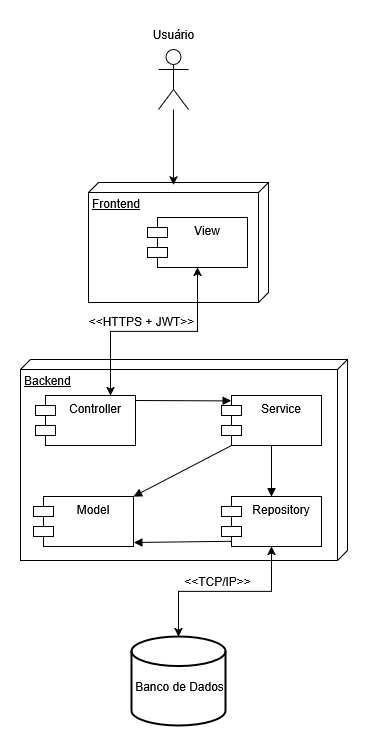
\includegraphics[height=0.5\textheight]{figuras/DIAGRAMA_IMPLANTACAO.png}
    \par
    Fonte: autoria própria com base em \cite{weissmann2014vire}.
    \par
    \label{arqprojeto)}
\end{figure}

\subsection{MVC (Model-View-Controller)}

O MVC é um padrão arquitetural que permite isolar completamente as camadas de negócio e visualização através de uma camada intermediária chamada controlador. Um problema recorrente que o MVC visa solucionar é o alto acoplamento do código, logo, a implementação do mesmo produz código com menos dependências, maior qualidade e testabilidade \cite{weissmann2014vire}. Isso ocorre pois as camadas são independentes entre si, ou seja, as camadas não possuem acesso direto entre si, o que torna a implementação da substituição das mesmas mais fácil.

Sendo assim, podemos descrever as funcionalidades das camadas da seguinte maneira. \textit{View} é a camada de apresentação para o usuário, onde o mesmo irá interagir com o sistema. No caso desse projeto, será o \textit{frontend}. As próximas duas camadas fazem parte do \textit{backend}, o \textit{Model} é a camada responsável por aplicar regras de negócios e consulta ao banco de dados. Por fim, o \textit{Controller} é responsável por intermediar a \textit{View} e \textit{Model}.


\subsection{Backend}  

O \textit{backend} representa o núcleo do sistema, sendo responsável por intemerdiar a comunicação entre o \textit{frontend} e o banco de dados. O mesmo, processa requisições, aplica regras de negócio, realiza validações e retorna a resposta para o usuário, garantindo operações de forma segura e autenticada no banco de dados. 

Ademais, para a organização de pastas, optou-se por adotar a separação entre camadas Controller, Service, Model e Repository, uma vez que, por convenção, projetos utilizando o Spring Framework costumam seguir essa estrutura, facilitando a integração com rcursos como Beans e ORMs, além de favorecer a manutenção e coesão \cite{weissmann2014vire}.

\begin{itemize}
    \item Controller - Controle de requisições da API RESTful.
    \item Service - Implementação de regras de negócio do sistema.
    \item Model - Entidades mapeadas do SGBDR.
    \item Repository - Interfaces de manipulação do SGBDR.
\end{itemize}

\subsubsection{API RESTful}

A comunicação do \textit{backend} com o \textit{frontend} será por meio das chamas \textit{Application Programming Interfaces Representational State Transfer} (APIs RESTful), especificamente as APIs RESTful utilizam o protocolo HTTP/1.1 como base para a comunicação entre cliente e servidor, utilizando o padrão de métodos \textit{get}, \textit{post}, \textit{delete} e \textit{put}, além disso, a troca de dados padrão envolve JSON (\textit{JavaScript Object Notation}).

Essa comunicação deve ser criptografada e autenticada, logo é importante a utilização do \textit{Transport Layer Security} (TSL) para criptografia e para a autorização é conveniente a utilização o Spring Security com suporte ao OAuth 2.0, visto que o mesmo permite a integração com provedores de identidade externos como Google, Facebook, entre outros. Também, é necessário a utilização do \textit{JSON Web Token} (JWT) para transferir tokens, de forma segura e compacta, contendo as informações de autorização e autenticação entre os sistemas \cite{nascimento_2017}. 

\subsubsection{Hibernate}

A fim de solucionar o alto acoplamento do código o Spring utiliza o DAO (\textit{Data Access Object}) que separa a lógica de acesso de dados da lógica de negócio da aplicação, em outras palavras o DAO oferece às classes clientes interfaces onde são expostas operações básicas como inserções, deleções e consultas. Essa lógica está separada em uma camada chamada \textit{Repository} \cite{weissmann2014vire}.

Ademais, um aspecto fundamental para manipulação de dados é a utilização de ORM (\textit{Object Relational Mapping}) no qual oferece a possibilidade de manipular entidades do SGBDR como objetos da POO (Programação Orientada a Objetos) \cite{weissmann2014vire}. Sendo assim, para esse projeto foi escolhido o Hibernate como provedor ORM devido a sua alta documentação e integração com o Spring.

\subsection{Frontend}

O \textit{frontend} é a camada de visualização e interação com o usuário. Por isso, é essencial que essa interface seja clara, intuitiva e eficiente. Para garantir isso, o modelo proposto segue as 10 heurísticas de usabilidade de Nielsen.

Em especial, é necessário que o sistema seja padronizado e acessível em diferentes dispositivos móveis, independente do sistema operacional. Sendo assim, optou-se por utilizar o React Native, um \textit{framework} que permite a criação de aplicações móveis multiplataforma.

\subsubsection{React Native}

React é uma biblioteca JavaScript baseada em componentes reutilizáveis, o que permite desenvolver sistemas recicláveis e independentes, favorecendo a manutenção e permitindo a escalabilidade \cite{boduch2017react}. 

Em suma, o React Native segue os mesmos princípios do React, porém, ao invés de gerar páginas \textit{web}, o React Native compila os componentes em elementos nativos, tanto para o Android quanto para o IOS (\textit{iPhone Operating System}). Sendo assim, o desempenho de aplicações em React Native é semelhante à utilização de linguagens nativas como Kotlin ou Swift \cite{boduch2017react}.